\chapter{Building Blocks: Basic Data Types}\label{chpt:building-blocks}

Chapter One outlines some basic datatypes and functional syntax used throughout the rest of the Book. Many of the function definitions herein use extremely loose syntax, which is all that's necessary for an introductory chapter. The only true reason this chapter exists is an exercise in rigor for those who enjoy such things, and a refresher course in basic concepts for those who may have forgotten. In other chapters, a level of knowledge consistent with mid-high school or higher will be assumed, and in even later chapters, an understanding of material in sections indicated at the beginning of those chapters.


\section{Functions}

Functions are incredibly useful constructs throughout mathematics, the natural sciences, and in particular
computer science. Functions take any number of inputs, or arguments, usually performing operations on those arguments to
produce an output. In mathematics in particular, a "function" is defined as having exactly one output value for any single set of input(s).

When writing the definition of a function, in will usually be given in a mathematical form, generally as being set equal to the expression that is the definition of the function. All functions are also presented using Python (3.10) code that you can type right into a Python file to define the same function using computer code. This section isn't meant to be an introduction to Python, but the syntax is so simple that in general the function definitions can be easily understood without any prior programming experience. However, as a simple explanation, the definition of a function in Python takes the form shown in Listing \ref{code:funcEx}. The same function defined in (somewhat) standard mathematical notation is shown in Equation \ref{func:functionname}.

\begin{listing}[H]
\caption{Function Example}\label{code:funcEx}
\begin{minted}{python}
def FunctionName(ArgName0: type, ArgName1: type, ... ArgNameN: type) -> ReturnType:
	Operations
	return Possible Output
\end{minted}
\end{listing}

\begin{equation}\label{func:funcname}
\textnormal{FunctionName}(ArgName_0, ArgName_1, \cdots ArgName_n) \coloneqq Expression \Longleftarrow
\end{equation}

As seen in Listing \ref{code:funcEx}, the first word is \code{def} which just tells Python that what follows will be a definition of a function (as opposed to e.g. a "class"). The second word is "FunctionName," which is a placeholder for the name of the function. A reader with any amount of experience with trigonometry will recognize the function name Sine (often stylized as "sin"), for example. When using a function, only the name of and arguments to the function need be provided for its use to be complete and valid. \\
After the function name, a list of comma-separated arguments, with their own "types" separated by colons, are specified. This "type" will be the name of the type of data that input to the function. In later chapters we will define more of these data-types, but for now we'll introduce the most simple. The end of the argument list is signified by a closing parenthesis, followed by the sequence \code{->} (meant to resemble an arrow) and the "return type" or "output type" of the function. It's important to note that \code{None} is the type of data that doesn't exist\footnote{Related concepts in other programming languages with which the reader may be familiar include \code{undefined}, \code{undef}, \code{null}, \code{void}, \code{nil}, and others. None of these are exactly the same as \code{None}, but they're all pretty close.}. That is to say, a function of type \code{None} not produce a result, and is typically used only in programming chapters, since it can't represent a valid mathematical function.
It should be noted that an argument cannot be of this type, as it's kind of nonsensical to pass no information as an argument. However, arguments \emph{can} be of a type that is "None OR some other type", to indicate that they may be optionally provided. Again, this is generally only possible as a programming function, but not a mathematical (or "pure") function.\\
A function may take any number of arguments, but the most common is simply one. In cases of multiple arguments the order of the arguments is important. A datum of type A may not be passed to a function that only accepts one argument of type B. Similarly, a function that takes one argument of type A, and then an argument of type B cannot be used on one argument of type B, and then an argument of type A. \\
\code{return} is used to specify that what follows is the output of the function. Traditionally, this is also the endpoint of the function. That is, any operations after it are ignored. For this reason, even functions that have the \code{None} type may return nothing (or explicitly \code{None}) to indicate that computation is to cease at that point, but it is certainly not required. \\
Functions are used in a similar manner to this throughout a few computer science languages. Specifically, those familiar with Ruby and GoDotScript may find Listing
\ref{code:funcEx} to be reminiscent of those languages.\\

Now, for those perhaps more familiar with Python than mathematics, the biggest differences between Equation \ref{func:funcname} and Listing \ref{code:funcEx} are
\begin{itemize}
	\item No types anywhere
	\item A single $Expression$ instead of room for an arbitrary number of sequential operations
	\item The use of $\coloneqq$ instead of \code{def} and indentation
\end{itemize}
Types in mathematics are rarely specified, and functions are simply understood to operate on some type. Generally in this text, the mathematical notation will avoid specifying types while the Python code samples will always specify them. When there is some ambiguity, or the types used are very unusual, the types are specified by specifying that an argument or the function's output are members of some set (see \ref{sec:sets} for information on what a "set" is). To get a bit ahead of ourselves, Equation \ref{func:typed-example} shows a sample function that has two inputs, $x$ and $y$, that are both "real numbers" (which are later described in \ref{sec:reals}) and an output that is also a "real number".\\
Unlike programming functions, mathematical functions aren't a series of steps to perform to do some kind of computing work. There is no host platform for math with which to interact (e.g. through \code{print}). Functions in mathematics are defined by declaring them to be equal to some expression. This means that while, in general, any mathematical function can be written in Python, there are infinite Python functions that cannot be expressed mathematically. A Python function can be written in mathematical notation if and only if it is a "pure function", meaning it operates on its inputs to provide a single output with no "side-effects" (e.g. printing to the console with \code{print}).\\
In mathematics, function definitions are widely done by just declaring that a function is equal to some expression. The symbol $\coloneqq$ used here may be unfamiliar even to some mathematicians, who would be more used to using $=$ in its place. This symbol is reserved for use as an expression mean "is equal to" in this text, and will never be used interchangeably with $\coloneqq$, which means "is defined as". Another similar symbol is $\equiv$, which means "is equivalent to" and will be covered later, but just note that it's also different from $\coloneqq$ and $=$. Some other symbols mathematicians may be used to that have the same meaning $\coloneqq$ include $\stackrel{\triangle}=$, $\stackrel{\text{def}}=$, and $\stackrel{\cdot}=$. These aren't used in this text; $\coloneqq$ was chosen to represent this concept.\\
More operators with similar meaning to equality and definition are given in \ref{sec:relational-operators}

\begin{equation}\label{func:typed-example}
\textnormal{FunctionName}(x\in\mathbb{R}, y\in\mathbb{R})\in\mathbb{R} \coloneqq x+y
\end{equation}

The way a function is used is called "calling" that function, and it takes the form shown in Listing \ref{code:funcCallEx}/Equation \ref{func:funcCallEx}.
\begin{listing}[H]
\caption{Example Function Call}\label{code:funcCallEx}
\begin{minted}{python}
FunctionName(Argument0, Argument1, ... ArgumentN)
\end{minted}
\end{listing}

\begin{equation}\label{func:funcCallEx}
\textnormal{FunctionName}(Argument_0, Argument_1, \cdots Argument_N)
\end{equation}

They're basically written the same way, and their usage is more or less also done the same way.

\section{Integers}
At this point it will be useful to define a data type that is not simply \code{None}. Many readers will already be familiar with the concept of integers, but this chapter exists largely for the purpose of rigorously defining perhaps somewhat simple ideas.\\


\subsection{Whole Numbers and the Successor Function}
Our starting point isn't to begin defining the integer, but to describe a new data type, the "whole number". The definition begins with one member from which all others are defined. That is to say:
\begin{center}
\textit{$0$ is the first whole number}
\end{center}

Python does not have an equivalent to the "whole number" type - the closest type would be \code{int}, which will in general be used in lieu of a proper type for whole numbers.

Don't worry about the definition of $0$'s value right now, that will become apparent shortly.\\
Every other whole number can be obtained from a recursive definition using the so-called "Successor Function" as shown in \ref{func:successor}, where a value with a subscript $n$ indicates the $n$th value and a function with a superscript $n$ indicates $n$ applications of said function. That is a little recursive, since counting is what's being defined, but it's being done anyway, just to save the space it would take up to write them manually (which would be infinite).
\begin{equation}\label{func:successor}
\textnormal{Whole Number}_n \coloneqq SuccessorFunction^n(0)
\end{equation}
This can also be expressed in the following way:
\begin{center}
$SuccessorFunction(0) = 1$\\
$SuccessorFunction(1) = 2$\\
Successor Function Example\label{eq:sucFuncEx}
\end{center}
This implies that the numbers $0$-$9$ are just symbols attributed to the whole numbers generated by by the Successor Function. It is commonplace to use what is known as a "base-ten number system," which means that upon reaching 9, two characters arise to take its place, starting with a $1$ in the furthest left, and a $0$ on the right. The place a number holds is called its digit. In general, whenever a digit that is 9 has the Successor Function called on it, the digit directly to the left has the Successor Function called on it, which increments the digit, and the digit that was $9$ becomes $0$. If there is no digit to the left, it is treated as $0$, which produces the whole number $1$ in that digit. Keep in mind that this is simply a way of representing an infinite number of outputs of the Successor Function, and as such should be thought of collectively as one whole number, not a collection of whole numbers. \\


\subsection{Addition}

It is easy to see at this point how simple arithmetic operations can be defined. The difference between operations and functions is largely immaterial, in fact it is useful to define operations as functions first, then show the symbol. For instance, addition can be described as shown in Equation \ref{eq:plusone}/Listing \ref{code:plusone}\footnote{Note that this assumes a working definition of \code{SuccessorFunction} - which wasn't provided. It's not possible to define the Successor Function in Python without either a recursive definition of addition or loss of sanity.}.
\begin{equation}\label{eq:plusone}
\textnormal{PlusOne}(x) \coloneqq SuccessorFunction(x) \equiv x+1
\end{equation}
\begin{listing}[H]
\caption{PlusOne Function}\label{code:plusone}
\begin{minted}{python}
def PlusOne(x: int) -> int:
	return SuccessorFunction(x)
\end{minted}
\end{listing}
So as seen above, adding one to a number is the same as calling the Successor Function on it (which may have been obvious by now). Then adding a number greater than one to some whole number $x$ is as simple as calling the successor function that many times. We can now easily define a symbol $+$ to represent calling the successor function x times on a whole number $y$ if given in the form $x+y$. At this point it is useful to note that
\begin{center}
$SuccessorFunction[2]=3=SuccessorFunction[SuccessorFunction[1]]$
\end{center}
which is a simple way of saying that $2+1=1+2$, known as the associative property of addition. \\
It is here that the value of $0$ becomes apparent. For example, consider the statement $1+0$. We know from above that this is equivalent to the statement \\ $SuccessorFunction[0]=1$. From here it is trivial to show that any whole number that has the number $0$ added to it retains its value.

\subsection{Negative Numbers and Subtraction}
Before going any further, we will develop our understanding of whole numbers into an understanding of integers. Like with whole numbers, the easiest place to start is with a function.
\begin{align}\label{func:predecessor}
\textnormal{PredecessorFunction}(x) \coloneqq y \\
\textnormal{such that SuccessorFunction}(y) = x
\end{align}

The Predecessor Function, it would seem, only undoes the Successor Function, and as such is sometimes called the Inverse Successor Function. Like with addition, it may be useful to think of the operation of subtraction as an implementation of the function defined in in Equation \ref{eq:minusone}/Listing \ref{code:minusone}\footnote{Note that this assumes a working definition of \code{PredecessorFunction} - which wasn't provided. It's not possible to define the Predecessor Function in Python without either a recursive definition of subtraction or loss of sanity.}.

\begin{equation}\label{eq:minusone}
\textnormal{MinusOne}(x) = PredecessorFunction(x) \equiv x-1
\end{equation}
\begin{listing}[H]
\caption{PlusOne Function}\label{code:minusone}
\begin{minted}{python}
def MinusOne(x: int) -> int:
	return PredecessorFunction(x)
\end{minted}
\end{listing}
The above function can be used to describe $x-1$, and in general subtraction of a whole number $x$ from a whole number $y$ is defined as calling the Predecessor Function x times on y, given the form $y-x$. \\
It is now easy to define all negative numbers as simply a number for which the operations of the Successor Function and the Predecessor Function are switched. That is to say that for a number $x$ and a number $y$, $y+x=y-$ "Negative $x$". There exists then a number $z$ for every $y$ such that $y+z=0$, which means that when adding the negative number $z$ to $y$, the Predecessor Function is called on $y$ exactly as many times as the Successor Function must be called on $0$ to obtain the value $y$. This is the definition of "Negative $y$", meaning $z=$"Negative $y$".\\
Because whole numbers obey the original definitions of addition and subtraction, these new negative numbers cannot be said to be whole numbers. The name of these new numbers, in conjunction with the whole numbers, is "integers". This type corresponds to Python's \code{int} type, and is denoted as a Set\footnote{See Section \ref{sec:sets}} using the symbol "$\mathbb{Z}$. \\
It is implied, of course, that this means that calling the Predecessor Function $x$ times on $0$ produces Negative $x$, that is to say that $0-1=$Negative $1$. Furthermore, because writing out "Negative" every time subtraction is used can get a bit cumbersome and cluttered, and because of their unique property that adding is subtracting and subtracting is adding, negative numbers are written in the notation
\begin{center}
Negative $x = -x$
\end{center}
This is because there is an implicit $0$ to the left of the $-x$, which is omitted simply because that too would get repetitive, and only the symbol '$-$' is required to indicate the negativity of an integer $x$. For integers, it can be seen that the statement $x-y$ is equivalent to the statement $x+$Negative $y = x+ -y$

\section{Sets}\label{sec:sets}
In mathematics, a set isn't so much a data-type as a way of organizing data. Strictly speaking, though, it in fact is a type in Python, named \code{set}. Sets most often contain homogeneous types of data, so the type is annotated with the type it contains e.g. the type of a set of integers is \code{set[int]}. Sets are useful throughout all fields of natural sciences, computer science, math and logic as a way of describing large (sometimes infinite) amounts of data. A set contains only information on the unique objects it contains, and not any information about the ordering thereof. For example, suppose I have a set A shown in Figure \ref{fig:setAEmpty}/Listing \ref{code:setAEmpty} that initially contains nothing, which incidentally has its own symbol: $\varnothing$.
\begin{center}
\begin{figure}[h]
\caption{Set A} \label{fig:setAEmpty}
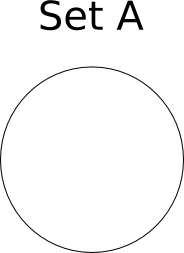
\includegraphics[scale=0.5]{figures/setAEmpty.png}
\end{figure}
\end{center}

\begin{listing}[H]
\caption{Definition of set A}\label{code:setAEmpty}
\begin{minted}{python}
A = {}
\end{minted}
\end{listing}

Now suppose I add the integer $1$ to set A - the resulting set is shown in Figure \ref{fig:setA1}/Listing \ref{code:setA1}.
\begin{center}
\begin{figure}[h]
\caption{Set A} \label{fig:setA1}
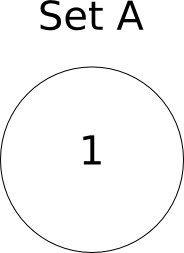
\includegraphics[scale=0.5]{figures/setA1.png}
\end{figure}
\end{center}

\begin{listing}[h]
\caption{Adding $1$ to set A}\label{code:setA1}
\begin{minted}{python}
A.add(1)
# A is now equivalent to this definition
A = {1}
\end{minted}
\end{listing}

If I were to try to add $1$ to set A again, Figure \ref{fig:setA1_0}/Listing \ref{code:setA1_0} shows what set A would look after I attempt that operation.

\begin{center}
\begin{figure}
\caption{Set A} \label{fig:setA1_0}
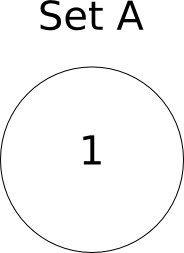
\includegraphics[scale=0.5]{figures/setA1.png}
\end{figure}
\end{center}

\begin{listing}[h]
\caption{Adding $1$ to set A a second time}\label{code:setA1_0}
\begin{minted}{python}
A.add(1)
# A is still equivalent to this definition
A = {1}
\end{minted}
\end{listing}

See, the set remains unchanged upon adding an element that it already contains. \emph{A set only contains information about the \textbf{unique} items it contains}. \\
Now suppose that I added the integer $2$ to this set - Figure \ref{fig:setA12}/Listing \ref{code:setA12} show the results of this operation.

\begin{center}
\begin{figure}
\caption{SetA} \label{fig:setA12}
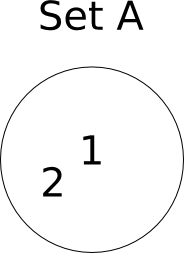
\includegraphics[scale=0.5]{figures/setA12.png}
\end{figure}
\end{center}

\begin{listing}[h]
\caption{Adding $1$ to set A}\label{code:setA12}
\begin{minted}{python}
A.add(2)
# A is now equivalent to this definition
A = {1, 2}
\end{minted}
\end{listing}

As seen above, there is no notion of the order or rank of the elements of A. Even though $1$ was added to the set before $2$, $1$ holds no special position, and the two integers are treated equally. There is a special, named set for the set that contains all whole numbers, denoted '$\mathbb{W}$', and the set that contains all integers, commonly denoted '$\mathbb{Z}$'.

\section{Lists and Tuples}
A list is extremely simple, it's something most readers are probably familiar with. In pedantic terms, a list is a collection of elements containing the information about which elements it contains (like a set), but also each element is associated with "ordinal" information. More simply put, a list is like a set, but order matters. A list is rarely if ever used in mathematics, but in Python it's an extremely useful construct, and has the type \code{list}. Like a set, a list usually contains a homogeneous type of data, and that type is expressed in a similar way e.g. the type of a list of integers is \code{list[int]}. The way a list is written is the same in mathematics as it is in Python. A list containing the first three whole numbers in order is written as $[0, 1, 2]$ while in Python it is represented \code{[0, 1, 2]}.\\

A tuple, on the other hand, is used extensively in mathematics, particularly in algebra (graphing) and linear algebra. Oddly enough a tuple is extremely similar to a list; it's just a group of values with ordinal information. The difference between the two is subtle, and largely semantic. In Python, the main difference is that a list's elements can change, while a tuple's cannot. The type of a tuple in python is simply \code{tuple}, and when it contains a homogeneous type of data the type can be expressed more precisely in much the same way as a list or a set e.g. a tuple of two integers has the type \code{tuple[int, int]}, a tuple of three integers has the type \code{tuple[int, int, int]}. Like lists, a tuple is written the same way in mathematics as it is in Python. For example, a tuple containing the first three whole numbers in order is written as $(0, 1, 2)$ and in Python as \code{(0, 1, 2)}.

Generally speaking the only real difference between these two is how they're used. A list typically represents \emph{successive} values, meaning values that are used in the same way one after the other e.g. in function input/output tables commonly used to help teach algebra. A tuple, on the other hand, almost always (at least in mathematics) contains \emph{orthogonal} values, as in a group of values that describe some concept that cannot be described as a single value e.g. a point in $\mathbb{R}^2$ like $(0, 1)$ which is pretty widely understood to be the point on an "x/y graph" at $x=0$ and $y=1$.

\subsection{Ranges}
A range can more or less be thought of as a kind of list. Technically speaking, in Python a range - which is represented by the type \code{range} - and a list are both \emph{iterable} values, though aren't actually any more related than that. Ranges are most commonly used when a list is desired of such length that it would be extremely tedious to write down all of the values.\\
Unlike lists and tuples, ranges aren't expressed the same way in mathematics as in Python. In mathematics, there are several ways to write ranges, depending on what you mean. A range is defined by its starting point, followed by its ending point, usually separated by a comma, but occasionally other textbooks use ellipses instead of a comma. The two values are surrounded by grouping symbols, one on the left that can be either $($ or $[$, and one on the right that can be either $)$ or $]$. A $[$ means "starting from and including", a $($ means "starting from but not including". Similarly, $]$ means "up to and including", while $)$ means "up to but not including". So, a range which encompasses all of the integers starting with $0$ and ending with $10$ may be written as $[0,10]$, $(-1,10]$, $[0,11)$, or $(-1,11)$ all equivalently (as long as it's known the values are integers - those are all very different ranges if the values are real or even just rational numbers!).\\
Python is much less flexible. In Python code, ranges are written as \code{range(start, end)} where \code{start} is \emph{always} included and end is \emph{always} excluded. Basically, the Python \code{range} type only allows the equivalent of the $[0,11)$ notation from the earlier example.

\section{Multiplication, Division and the Order of Operations}
Before we can continue to build up sets of useful constructs, we first need to define some more operations that can be preformed on integers (specifically division will be of interest later). \\

\subsection{Multiplication}
Of the two operations that make up the title of this section, multiplication is the easier of the two to explain. The function "Multiply" shown in Equation \ref{func:multiply}/Listing \ref{code:multiply} describe it in loose terms.

\begin{equation}\label{func:multiply}
\textnormal{Multiply}(x, y) = \sum^yx
\end{equation}

\begin{listing}[H]
\caption{Multiply Function}\label{code:multiply}
\begin{minted}{python}
# Python's built-in operator for multiplication is
# '*', so 'Multiply(x,y)' is equivalent to 'x*y'.
def Multiply(x: int, y: int) -> int:
	result = 0
	for xn in range(0, y):
		result = result + x
	return result
\end{minted}
\end{listing}

What this means, in English, is that multiplying $x$ by $y$ returns $x$ added to $x$ $y$ times. For this reason, expressions of the form $x\times y$ are typically pronounced "$x$ times $y$", and the '$\times$' symbol denotes multiplying the left side by the right side. This is often abbreviated, as the $\times$ symbol can be confused with a variable named $x$, as simply $xy$. That is not valid in Python, where the \code{*} operator may not be omitted in multiplication.\\

Multiplication of a number by itself repeatedly is represented in a special way called a 'power'. A power is written with the number of times the base number (appropriately called the 'base') written to the upper-right as a superscript (called the 'exponent'). The following function describes it in a similar way that multiplication was explained in \ref{code:multFunc}. Some interesting properties of powers are that $X^0=1$ for every $x$ of integer type (and actually all real and complex $x$, but those types of numbers will be discussed later), and $x^{-y}=\frac{1}{x^y}$.

\begin{equation}\label{func:power}
\textnormal{Power}(x, y) = \prod^yx
\end{equation}

\begin{listing}[H]
\begin{minted}{python}
# Python's built-in operator for powers is
# '**', so 'Power(x,y)' is equivalent to 'x**y'.
def Power(x: int, y: int) -> int:
	result = 0
	for xn in range(0, y):
		result = result * x
	return result
\end{minted}
\end{listing}
The invocation of this function is written in the form '$x^y$' in mathematics, where $x$ is being multiplied by itself $y$ times, also called 'raising $x$ to the $y$ power'. Note, though, that many mathematical disciplines and fields of focus tend to also use the same kind of relative symbol positioning for concepts not at all related to powers or multiplication.

\subsection{Order of Operations}
There are some more properties of multiplication that are necessary to understand division in base ten format, but these cannot be discussed without first knowing the Order of Operations. This is a set of rules for what order in which operations are to be performed, otherwise an expression written by one mathematician could be evaluated differently by another mathematician. The Order of Operations is:
\begin{center}
\begin{enumerate}
	\label{enum:OrderOps}
	\item{Function Calls}
	\item{Grouping Symbols}
	\item{Exponents}
	\item{Multiplication and Division}
	\item{Addition and Subtraction}
\end{enumerate}
\end{center}
The order in which these items are placed reflects their priority. For example, given the function definition in Equation \ref{func:plusfive}

\begin{equation}\label{func:plusfive}
\textnormal{PlusFive}(x)=x+5
\end{equation}

and the expression $10 + 2 \times 4 + PlusFive(3)-10+(2-2^2)$ it might be confusing what the value of the output is without having a canonical way of deciding which operations take precedence over others. In this example, we first look for function calls, and we find PlusFive$(3)$. Once that is evaluated, the expression becomes $10+2\times 4+ 8 -10+(2-2^2)$. From here, we must next look for grouping symbols, and the ones we find are those parenthesis. Parenthesis are grouping symbol whose only function is to indicate that the expression within them are to be indicated before the expressions outside them. In this case that expression is $2-2^2$. There are no functions in this expression, so we evaluate the power first, which leaves $2-4$. There's only one operation left, and that leaves $-2$. Now we replace the original grouping symbols with this output: $10+2\times 4+8-10-2$. After grouping symbols, we do multiplication and division from left to right. There's only one multiplication, $2\times 4$, and no division, so evaluating this and placing the output where the operation was leaves only $10+8+8-10-2$ remaining. All that's left is addition and subtraction, resulting in a final output of $14$.

\subsection{Division}
To put it as simply as possible, division is the operation that undoes multiplication. However, similar to subtraction, order matters. For instance, if $z$ is the output of $x\times y$, then the output of dividing $z$ by $x$ is $y$. Similarly, the output of $z$ divided by $y$ is $x$. Because order matters, dividing $y$ by $z$ is \emph{not} the same as dividing $z$ by $y$.\\

There are, however, many cases where there is no integer that $y$ can be multiplied by to obtain $x$. Consider, for example, the division of $5$ by $3$ (there is no integer $y$ such that $y$ times 3 outputs 5). In these cases, the output is left in the form of what is known as a 'fraction'. Fractions take the form $\frac{x}{y}$ or $x/y$ when dividing $x$ by $y$. The difference between them is accounted for by the versatility of the environment in which it is written, $\frac{x}{y}$ is the preferred form, but $x/y$ may be used when such typesetting is unavailable. \\
In a base ten number system, it becomes bothersome to always write fractions this way, but to understand it we must first describe some properties of fractions. \\
The value of a fraction is invariant under multiplication of both the top (called the 'numerator') and the bottom (called the 'denominator') by the same integer. Because division is merely the inverse of multiplication, the same must be true for division.

\begin{equation}
x / y = \frac{x}{y} = \frac{x\times c}{y \times c} = \frac{x / c}{y / c}
\end{equation}

The fraction is also a type of grouping symbol, which can be useful to avoid clutter caused by parenthesis. This means that
\begin{equation}
\frac{x+y}{a+b}
\end{equation}

is equivalent to

\begin{equation}
(x+y)/(a+b)
\end{equation}

for all $x$, $y$, $a$ and $b$. Also, because it's a grouping symbol, any valid expression can exist in either the numerator or the denominator. This means that fractions can be nested, like in Equation \ref{eq:fraction-nesting}.

\begin{equation}\label{eq:fraction-nesting}
a / \left(\frac{b}{c}\right) =\frac{a}{\left(\frac{b}{c}\right)} = \frac{a}{\frac{b}{c}}
\end{equation}

In Python, fractions are not a native type. All division must be expressed using the division operator "\code{/}" (or the related "floor division" operator \code{//} or the \code{divmod} function) and grouping parenthesis as necessary. It would be very simple to create a type that can represent a fraction, although it would be lengthy to get it to accept all of the standard mathematical operators that other numbers like \code{int}s support.

In a base ten system, these fractions are to be converted to fractions of ten in whatever way is available. For example, $\frac{2}{5}$ can be multiplied by $2$ on the top and bottom to obtain $\frac{4}{10}$ and the fraction $\frac{12}{30}$ can be divided by $3$ on the top and bottom to obtain $\frac{4}{10}$. This fraction can then be represented in the form $0.4$. As may be apparent by now, the base ten system is very closely tied with powers of ten. A number in the first digit is multiplied by $10^0$ (called the "one's" place'), the second digit is multiplied by $10^1$, the third by $10^2$ and so on, then these products are added which gives the full value of the number. When representing fractions in base ten format, a '.' called a decimal point (or sometimes radix point to generalize between base systems) is placed behind the one's place, and to the right of it fractions of $10^{-1}$ are represented without the denominator. This is continuously true for all negative powers of ten, that is to say that two places to the right of the decimal point are fractions of $10^{-2}$, three places to the right lie fractions of $10^{-3}$ and so on. Here are some examples:
\begin{center}
$1+\frac{7}{10}=1.7$ \\
$3+\frac{1}{20}=3+\frac{5}{100}=3.05$ \\
$1+\frac{6}{25}=1+\frac{24}{100}=1.24$ \\
\end{center}
In general, many fractions can be expressed this way because the negative powers of ten keep going to infinity, so even fractions of arbitrarily large denominators can be expressed. Decimal numbers are the preferred way of representing output values in most fields of computing, and fractions are only used to indicate division. By contrast, in algebra it's often impossible to reduce fractions beyond a certain point, because they involve unknown quantities, and any decimal number in mathematics is generally regarded as a mere approximation while fractions are exact. The set of all integers and all fractions that can be represented as a decimal number forms a special set called the 'Rational Numbers,' and it has its own special symbol: $\mathbb{Q}$.

\subsection{Real Numbers}\label{sec:reals}
There is only one step left before the most useful basic data type is defined. Consider a fraction such as $\frac{1}{3}$. This number cannot be expressed as any multiple of any negative power of ten. It is recursively just a little bit bigger than $\frac{3}{10}$, $\frac{33}{100}$, $\frac{333}{1000}$ and so on. However, it's always closer to a numerator constructed of repeating digits of $3$ than one that is constructed of repeating $3$'s that end in a $4$. For this reason, the decimal system can make an approximation that takes the form of $0.33333333333333333333\ldots$ and so on to infinity, which is abbreviated as $0.\overline{3}$. Any fraction that cannot be represented as a decimal, but can be approximated as an infinitely repeating decimal, is also considered a rational number, because it can be represented as a fraction. Actually, any number that can be represented as a fraction is a rational number. There are, however, some natural numbers that defy representation as a fraction or repeating decimal. Examples include $\pi$, $\sqrt{2}$, and $e$, these numbers have values that never repeat, and cannot be represented as a fraction, and only approximations to them can be made in a base ten system. This class of number is called "Irrational," and the set of all numbers that are irrational has the special symbol $\mathbb{I}$. Numbers such as pi are known due to certain relationships in nature (in pi's case the ratio of a perfect circle's diameter to its circumference), and so must be considered a part of the numbers we work with. After all, the value $4$ cannot be added to the color blue. Similarly, a rational number cannot be added to one of these irrational numbers. Unless, that is, a larger set is constructed of the elements of both the rational and irrational numbers. This large set that composes most numbers dealt with in algebra and calculus is called the 'Real Numbers,' and it has the special symbol $\mathbb{R}$.\\
The (rough) equivalent of real numbers in Python is the \code{float} type. Due to limitations of computing, the actual values that a \code{float} can hold are finite, and all can be represented as some decimal that either repeats or terminates. So technically, \code{float}s only ever contain rational values. However, that's a limitation of the hardware that runs Python, not something defined as a limitation in the language itself. On a system that can actually store irrational values somehow (which would require infinite memory on classical computing systems), Python would happily expose those values as a \code{float}, and so for the purposes herein, that type is treated as equivalent to $\mathbb{R}$.























